\documentclass{unicamthesis}


\usepackage{tikz}
\usetikzlibrary{automata, positioning}
\usepackage{lipsum}
\usepackage{booktabs}
\usepackage{cite}


\title{Title of your thesis here}
\author{Will Smith}
\coursename{Computer Science}
\curriculumname{Blockchain And Digital Ledger Technology}
\cyclenumber{XXXVIII}
\supervisorname{Prof. XXXXX}
\cosupervisorname{Prof. YYYYY}
\coordinatorname{Prof. ZZZZZ}
\dateofaward{Dec 2025}

\begin{document}

\maketitle
\printcolophon

\begin{declaration}
	I hereby declare that this thesis is my own work and has not been submitted elsewhere for any academic purpose.
\end{declaration}

\begin{abstract}
	\lipsum[1]
\end{abstract}
\newpage

\tableofcontents
\listoffigures\addcontentsline{toc}{chapter}{List of Figures}
\listoftables\addcontentsline{toc}{chapter}{List of Tables}
\listofalgorithms\addcontentsline{toc}{chapter}{List of Algorithms}

\cleardoublepage
\part{Prologue}

\chapter{Introduction}
\section{Context}
\lipsum[2]

\section{Motivation}
\lipsum[3]

\chapter{Background}
\section{Finite State Machines}
Here is a simple FSM diagram using TikZ:

\begin{figure}[ht]
	\centering
	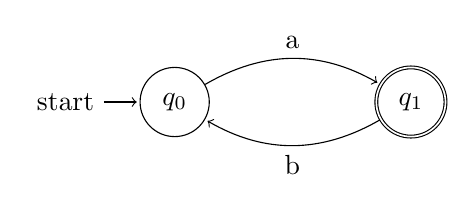
\begin{tikzpicture}[shorten >=1pt, node distance=3cm, on grid, auto]
		\node[state, initial] (q_0) {$q_0$};
		\node[state, accepting] (q_1) [right=of q_0] {$q_1$};
		\path[->]
		(q_0) edge [bend left] node {a} (q_1)
		(q_1) edge [bend left] node {b} (q_0);
	\end{tikzpicture}
	\caption{Example FSM for binary input}
	\label{fig:fsm}
\end{figure}

\section{Definitions and Examples}
\begin{definition}
	A finite state machine is a 5-tuple $(Q, \Sigma, \delta, q_0, F)$ where:
	\begin{itemize}
		\item $Q$ is a finite set of states~\cite{permenev2020verx,mavridouL18fsolidm}.
		\item $\Sigma$ is a finite set of input symbols.
		\item $\delta : Q \times \Sigma \to Q$ is the transition function.
		\item $q_0 \in Q$ is the initial state.
		\item $F \subseteq Q$ is the set of accepting states.
	\end{itemize}
\end{definition}

\begin{example}
	Let $Q = \{q_0, q_1\}$, $\Sigma = \{a, b\}$, and $\delta$ as shown in Figure~\ref{fig:fsm}. This FSM accepts alternating inputs.
\end{example}

\chapter{Results}
\section{A Table of Parameters}

\begin{table}[ht]
	\centering
	\begin{tabular}{@{}lll@{}}
		\toprule
		Parameter & Value & Description \\
		\midrule
		$\alpha$ & 0.05 & Learning rate \\
		$\beta$ & 0.9 & Discount factor \\
		$n$     & 1000 & Epochs \\
		\bottomrule
	\end{tabular}
	\caption{Experimental parameters}
	\label{tab:params}
\end{table}

\section{Discussion}
As shown in Table~\ref{tab:params}, the selected hyperparameters are suitable for convergence. More experiments are needed.

\chapter{Conclusion}
\lipsum[4-5]


\bibliographystyle{plain}
\bibliography{bib}
\end{document}
